\documentclass[journal,12pt,onecolumn]{IEEEtran}
\usepackage{amsmath,amssymb,amsfonts,amsthm}
\usepackage{graphicx}
\usepackage{enumitem}
\usepackage{multicol}
\usepackage[breaklinks=true]{hyperref}
\usepackage{caption}
\usepackage{amsmath}
\newtheorem{problem}{Problem}
\renewcommand{\thefigure}{\theenumi}
\renewcommand{\thetable}{\theenumi}
\newcommand{\myvec}[1]{\begin{pmatrix}#1\end{pmatrix}}

\begin{document}

\title{GATE XE 2011}
\author{AI25BTECH11003 - Bhavesh Gaikwad}
\maketitle

\section*{General Aptitude (Compulsory)}
\vspace{1cm}
\begin{enumerate}[label=\textbf{Q\arabic*.},itemsep=2em]

\item Choose the most appropriate word from the options given below to complete the following sentence: \\
Under ethical guidelines recently adopted by the Indian Medical Association, human genes are to be manipulated only to correct diseases for which treatments are unsatisfactory.\\

\hfill{(GATE 2011 XE)} \\
\begin{multicols}{4}
(A) similar 
(B) most 
(C) uncommon 
(D) available
\end{multicols}

\item Choose the word from the options given below that is most nearly opposite in meaning to the given word: Frequency\\

\hfill{(GATE 2011 XE)} \\
\begin{multicols}{4}
(A) periodicity \\
(B) rarity \\
(C) gradualness \\
(D) persistency
\end{multicols}

\item Choose the most appropriate word from the options given below to complete the following sentence: \\
It was her view that the country's problems had been so that to invite them to come back would be counter-productive. \\

\hfill{(GATE 2011 XE)} \\
\begin{multicols}{4}
(A) identified \\
(B) ascertained \\
(C) exacerbated \\
(D) analysed
\end{multicols}

\item There are two candidates P and Q in an election. During the campaign, 40\% of the voters promised to vote for P, and rest for Q. However, on the day of election 15\% of the voters went back on their promise to vote for P and instead voted for Q. 25\% of the voters went back on their promise to vote for Q and instead voted for P. Suppose, P lost by 2 votes, then what was the total number of voters?\\
\hfill{(GATE 2011 XE)} \\
\begin{multicols}{4}
(A) 100 \\
(B) 110 \\
(C) 90 \\
(D) 95
\end{multicols}

\newpage

\item The question below consists of a pair of related words followed by four pairs of words. Select the pair that best expresses the relation in the original pair: \\
Gladiator: Arena \\

\hfill{(GATE 2011 XE)} \\
\begin{multicols}{4}
(A) dancer: stage \\
(B) commuter : train \\
(C) teacher: classroom \\
(D) lawyer: courtroom
\end{multicols}

\item The sum of n terms of the series 4+44+444+.... is \\

\hfill{(GATE 2011 XE)} \\
\begin{multicols}{4}
(A) $\frac{4}{81} [10^{n+1} - 9n - 1]$ \\
(B) $\frac{4}{81} [10^{n-1} - 9n - 1]$ \\
(C) $\frac{4}{81} [10^{n+1} - 9n - 10]$ \\
(D) $\frac{4}{81} [10^{n} - 9n - 10]$
\end{multicols}


\item Given that f(y)=$\frac{|y|}{y}$, and q is any non-zero real number, the value of $|f(q) - f(-q)|$ is \\

\hfill{(GATE 2011 XE)} \\
\begin{multicols}{4}
(A) 0 \\
(B) -1 \\
(C) 1 \\
(D) 2
\end{multicols}

\item Three friends, R, S and T shared toffee from a bowl. R took 1/3rd of the toffees, but returned four to the bowl. S took 1/4th of what was left but returned three toffees to the bowl. T took half of the remainder but returned two back into the bowl. If the bowl had 17 toffees left, how many toffees were originally there in the bowl? \\

\hfill{(GATE 2011 XE)} \\
\begin{multicols}{4}
(A) 38 \\
(B) 31 \\
(C) 48 \\
(D) 41
\end{multicols}

\newpage

\item The fuel consumed by a motorcycle during a journey while traveling at various speeds is indicated in the graph below.

\begin{figure}[h]
\centering
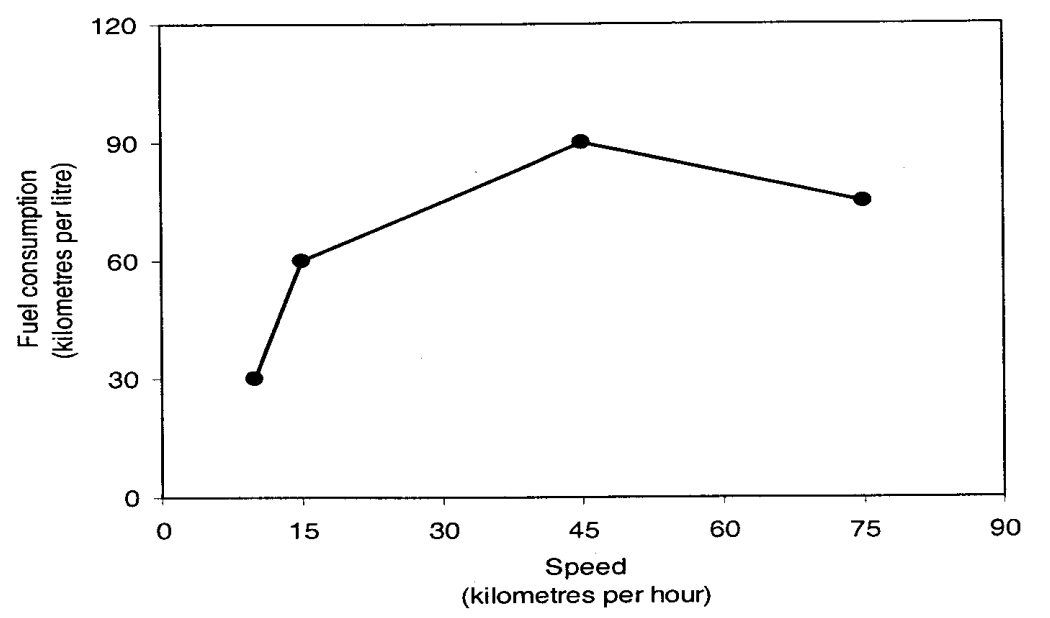
\includegraphics[width=0.5\columnwidth]{figs/GA/fig1.png}
\caption{Fuel consumption graph}
\label{fig:figs/GA/fig1.png}
\end{figure}

The distances covered during four laps of the journey are listed in the table below:\\

\begin{tabular}[12pt]{ |c| c| } 
    \hline
    {Group I: Aircraft mode} & {Group II: Property}\\ 
    \hline
    P: Short period mode & 1: Coupled roll-yaw oscillations\\
    \hline 
    Q: Wing rock & 2: Angle of attack remains constant \\
    \hline
    R: Phugoid mode & 3: Roll oscillations \\
    \hline   
    S: Dutch roll & 4: Speed remains constant\\
    \hline
\end{tabular}


From the given data, we can conclude that the fuel consumed per kilometre was least during the lap \\

\hfill{(GATE 2011 XE)} \\
\begin{multicols}{4}
(A) P \\
(B) Q \\
(C) R \\
(D) S
\end{multicols}

\item The horse has played a little known but very important role in the field of medicine. Horses were injected with toxins of diseases until their blood built up immunities. Then a serum was made from their blood. Serums to fight with diphtheria and tetanus were developed this way. It can be inferred from the passage, that horses were \\

\hfill{(GATE 2011 XE)} \\
\begin{multicols}{4}
(A) given immunity to diseases \\
(B) generally quite immune to diseases \\
(C) given medicines to fight toxins \\
(D) given diphtheria and tetanus serums
\end{multicols}


\vspace{3\baselineskip}
    \begin{center}
    \textbf{\Large END OF SECTION- GA}
    \end{center}
    
\end{enumerate}

%---------------Section-A------------------
\clearpage
\section*{A: Engineering Mathematics (Compulsory)}
\begin{enumerate}[label=\textbf{Q\arabic*.},itemsep=2em]
\vspace{1cm}

\item A vector field is called solenoidal if its divergence is zero. Consider the vector fields P and Q given by \\
P(x, y, z) = (2x² + 8xy²z) i + (3x²y - 3xy) j - (4y²z² + 2xz) k and \\
Q(x, y, z) = xyz² P(x, y, z). Then \\

\hfill{(GATE 2011 XE)} \\
\begin{multicols}{2}
(A) P and Q are both solenoidal \\
(B) both P and Q are not solenoidal \\
(C) P is solenoidal but not Q \\
(D) Q is solenoidal but not P
\end{multicols}

\item The eigenvalues of a 3×3 matrix P are 2, 2 and -1. Then $P^{-1}$ is equal to \\

\hfill{(GATE 2011 XE)} \\
\begin{multicols}{4}
(A) $3P - P^2$ \\
(B) $P^2 - 2P$ \\
(C) $P^2 + 3P$ \\
(D) $P^2 + 2P$
\end{multicols}

\item The integral $\int e^x \sin^2 x \, dx$ equals \\

\hfill{(GATE 2011 XE)} \\
\begin{multicols}{4}
(A) 4 \\
(B) 0 \\
(C) 8 \\
(D) 2
\end{multicols}

\item The integral $\oint_C \frac{(2z-1)^3}{z} dz$ along curve $C: |z| = 1$, oriented counter-clockwise, equals \\

\hfill{(GATE 2011 XE)} \\
\begin{multicols}{4}
(A) $2\pi i$ \\
(B) $20\pi i$ \\
(C) $13\pi i$ \\
(D) 0
\end{multicols}

\item Consider the function $f(x,y,z) = x^3 e^{\sin z}$ and the point $P = (1,0, \frac{\pi}{2})$. The value of f does not change due to a small displacement of P along the direction of \\

\hfill{(GATE 2011 XE)} \\
\begin{multicols}{4}
(A) $[1,0,\pi/2]$ \\
(B) $[1,-1,1]$ \\
(C) $[1,-3,0]$ \\
(D) $[2,0,-1]$
\end{multicols}

\newpage

\item A solution of the differential equation $\frac{d^2 y}{dx^2} - 5 \frac{dy}{dx} + 6y = 36x$ is \\

\hfill{(GATE 2011 XE)} \\
\begin{multicols}{4}
(A) $e^{2x} + e^{3x} + 6x + 5$ \\
(B) $e^x + e^{-3x} + 6x + 5$ \\
(C) $e^{2x} + e^{-3x} + 6x + x$ \\
(D) $e^{2x} + e^{3x} + x + 5$
\end{multicols}

\item For any positive numbers a and b, the matrix 
$P = a\myvec{4 & 5 & 6 \\ 5 & 4 & 6}$ is \\

\hfill{(GATE 2011 XE)} \\
\begin{multicols}{4}
(A) orthogonal \\
(B) diagonalizable \\
(C) nonsingular \\
(D) of rank 2
\end{multicols}

\item Suppose x is the nth iterated value while finding the positive square root of 7 by the Newton-Raphson method with a positive initial guess $x \neq \sqrt{7}$. If $e_n = \sqrt{7} - x$, for $n \geq 1$, then \\

\hfill{(GATE 2011 XE)} \\
\begin{multicols}{4}
(A) $e_{n+1} = \frac{2}{n} e_n^2$ \\
(B) $e_{n+1} = \frac{1}{2} e_n$ \\
(C) $e_{n+1} = \frac{\sqrt{5}}{2} e_n$ \\
(D) $e_{n+1} = e_n$
\end{multicols}

\item The solution of the initial boundary value problem with $\frac{\partial u}{\partial t} = \frac{\partial^2 u}{\partial x^2}$, $0 < x < \pi, t > 0$, with boundary conditions $u(0,t)=0 = u(\pi, t)$ and initial condition $u(x,0) = f(x)$, is \\

\hfill{(GATE 2011 XE)} \\
\begin{multicols}{2}
(A) $u(x,t) = 2 A_n \exp(-n^2 t) \cos(nx)$ with $A_n = \frac{2}{\pi} \int_0^{\pi} f(x) \cos(nx) dx$ \\
(B) $u(x,t) = \sum A_n \exp(-n^2 t) \cos(nx)$ with $A_n = \frac{2}{\pi} \int_0^{\pi} f(x) \cos(nx) dx$ \\
(C) $u(x,t) = \sum A_n \exp(-n^2 t) \sin(nx)$ with $A_n = \frac{2}{\pi} \int_0^{\pi} f(x) \sin(nx) dx$ \\
(D) $u(x,t) = \sum A_n \exp(-n^2 t) \sin(nx)$ with $A_n = \frac{2}{\pi} \int_0^{\pi} f(x) \sin(nx) dx$
\end{multicols}

\item The function f(x) defined by
\begin{align} 
f(x) = 
\begin{cases} 
3 - x^2, & x \leq 1, \\
3 - x, & 1 < x \leq 2, \\
x - 1, & x > 2,
\end{cases}
\end{align}
has\\ 

\hfill{(GATE 2011 XE)} \\\
\begin{multicols}{2}
(A) a local maxima at x = 3 and a local minima at x = 0 \\
(B) a local maxima at x = 0 and no local minima \\ 
(C) a local maxima at x = 0 and a local minima at x = 2 \\
(D) no local maxima and a local minima at x = 1
\end{multicols}


\item In a biased die experiment, the random variable x of the outcome has the (cumulative) distribution function F(x) as shown below.

\begin{figure}[htbp]
  \centering
  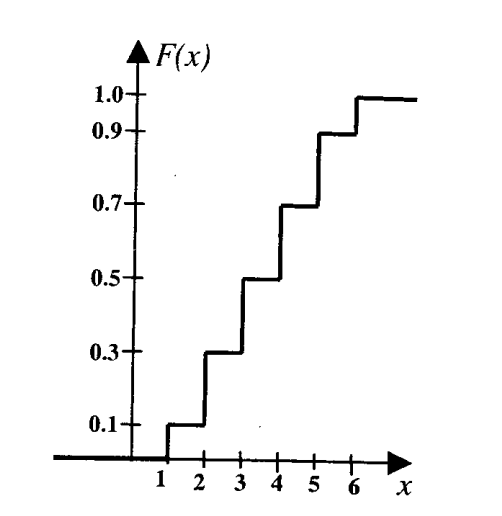
\includegraphics[width=.6\columnwidth]{figs/A/fig1.png}
  \caption{Graph}
  \label{fig:figs/A/fig1.png}
\end{figure}


The variance of x is\\

\hfill{(GATE 2011 XE)} \\
(A) 1.5 
(B) 2.25 
(C) 3.5   
(D) 4.25   

\vspace{3\baselineskip}
    \begin{center}
    \textbf{\Large END OF SECTION- A}
    \end{center}

\end{enumerate}


%----------------SECTION-B---------------------
\newpage
\section*{B: Fluid Mechanics}
\vspace{1cm}
\begin{enumerate}

\item For a boundary layer on a flat plate, \_\_\_ forces and \_\_\_ forces are of the same order of magnitude.\\

\hfill{(GATE 2011 XE)} \\
\begin{multicols}{4}
(A) body, inertia\\
(B) viscous, body\\
(C) inertia, viscous\\
(D) viscous, pressure
\end{multicols}

\item The temperature field in a fluid flow is given by $(60 - 0.2 x y)^\circ$C. The velocity field is ${\bf V} = 2 x y\, \mathbf{i} + t y\, \mathbf{j}$ m/s. The rate of change of the temperature measured by a thermometer moving along with the flow at (2, 4) m at $t=4$ s is\\

\hfill{(GATE 2011 XE)} \\
\begin{multicols}{4}
(A) $-12.8^\circ$C/s\\
(B) $-10.6^\circ$C/s\\
(C) $-6.4^\circ$C/s\\
(D) $-4.8^\circ$C/s
\end{multicols}

\item Two tanks, A and B, with the same height are filled with water till the top. The volume of tank A is 10 times the volume of tank B. What can you say about the pressures $P_A$ and $P_B$ at the bottom of the tanks A and B respectively?\\

\hfill{(GATE 2011 XE)} \\
\begin{multicols}{2}
(A) $P_A = 10 P_B$\\
(B) $P_B = 10 P_A$\\
(C) $P_A = P_B$\\
(D) Additional data is required to compare the two pressures.
\end{multicols}

\item A velocity field in a plane flow is given by ${\bf V} = 2 x y\, \mathbf{i} + 3 y\, \mathbf{j}$ m/s. The vorticity at the point (2, 4) m is\\

\hfill{(GATE 2011 XE)} \\
\begin{multicols}{4}
(A) $-4\, \mathbf{k}$ rad/s\\
(B) $3\, \mathbf{j}$ rad/s\\
(C) $2\, \mathbf{k}$ rad/s\\
(D) $-3\, \mathbf{i}$ rad/s
\end{multicols}

\item Separation is said to occur at a wall when at the wall \_\_\_\_ becomes zero.\\

\hfill{(GATE 2011 XE)} \\
\begin{multicols}{4}
(A) internal energy\\
(B) pressure\\
(C) shear stress\\
(D) density
\end{multicols}

\newpage

\item A certain fluid flow is influenced by density $(\rho)$, angular velocity $(\omega)$, dynamic viscosity $(\mu)$, and a characteristic length $(L)$. A relevant non-dimensional parameter will be\\
\hfill{(GATE 2011 XE)} \\
\begin{multicols}{4}
(A) $\rho \omega \mu / L^2$\\
(B) $\rho \omega L^2 / \mu$\\
(C) $\rho \omega \mu L$\\
(D) $\rho \omega \mu L$
\end{multicols}

\item The drags due to potential flow past a cylinder of diameter D cm and a slender airfoil of chord length D cm are compared. Assuming unit depth for both the bodies, which one of the following would be TRUE?\\
\hfill{(GATE 2011 XE)} \\
\begin{multicols}{2}
(A) The drag on the cylinder is greater\\
(B) The drag on the airfoil is greater\\
(C) Both the drags are equal\\
(D) Additional data is needed to compare the drags
\end{multicols}

\item For a fully developed flow between two parallel flat plates, the velocity gradient at a point is found to be 1000 s$^{-1}$. If the density of the fluid is 880 kg/m$^3$ and the kinematic viscosity of the fluid is $7.4 \times 10^{-7}$ m$^2$/s, the shear stress at the same point is approximately\\

\hfill{(GATE 2011 XE)} \\
\begin{multicols}{4}
(A) 0 Pa\\
(B) 1.30 Pa\\
(C) 0.32 Pa\\
(D) 0.65 Pa
\end{multicols}

\item An open channel flow is to be simulated in the laboratory. For this purpose, a 1:25 scale model is constructed. If the flow velocity in the prototype is 5 m/s, for dynamic similarity the model should have a flow velocity of\\

\hfill{(GATE 2011 XE)} \\
\begin{multicols}{4}
(A) 5 m/s\\
(B) 1 m/s\\
(C) 125 m/s\\
(D) 25 m/s
\end{multicols}

\item A pitot-static probe is inserted in an air flow. A manometer connected to this probe having Hg as the manometric fluid shows a difference of 30 mm. Assume a probe factor of 1. Assuming $\rho_{air} = 1.23$ kg/m$^3$, $\rho_{Hg} = 13,600$ kg/m$^3$ and $g = 10$ m/s$^2$, the speed of the air flow is approximately\\

\hfill{(GATE 2011 XE)} \\
\begin{multicols}{4}
(A) 66.5 m/s\\
(B) 81.5 m/s\\
(C) 76.5 m/s\\
(D) 92.5 m/s
\end{multicols}

\newpage

\item Consider an L-shaped gate with water level above the hinge as shown. At approximately what height $D$ of the water level will the gate open? Neglect the mass of the gate. Assume $g = 10$ m/s$^2$.\\

\begin{figure}[htbp]
  \centering
  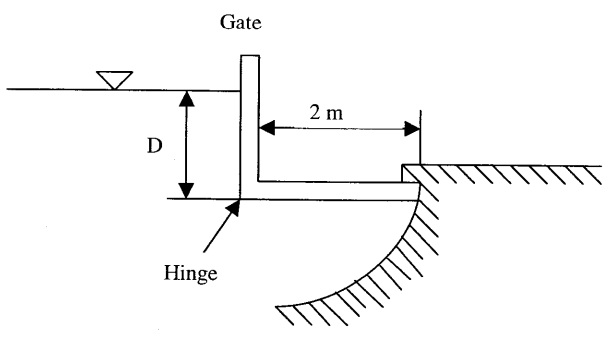
\includegraphics[width=.65\columnwidth]{figs/B/fig1.png}
  \caption{Diagram}
  \label{fig:figs/B/fig1.png}
\end{figure}


\hfill{(GATE 2011 XE)} \\
\begin{multicols}{4}
(A) 3.46 m\\
(B) 4.36 m\\
(C) 6.43 m\\
(D) 5.36 m
\end{multicols}

\item When a large tank containing water is placed on a weighing scale, a reading of 10000 N is obtained. The tank is fitted with an outlet pipe and a valve as shown. When the valve is opened, a jet of water with a velocity of 10 m/s issues out in the vertically upward direction. The diameter of the outlet pipe is 10 cm. Determine approximately the reading on the weighing scale at the instant the valve is opened and the water jet issues out. Density of water is 1000 kg/m$^3$.\\

\begin{figure}[htbp]
  \centering
  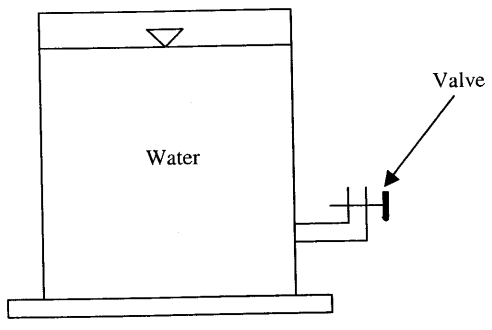
\includegraphics[width=.35\columnwidth]{figs/B/fig2.png}
  \caption{Large Tank Diagram}
  \label{fig:figs/B/fig2.png}
\end{figure}

\hfill{(GATE 2011 XE)} \\
\begin{multicols}{4}
(A) 9215 N\\
(B) 10000 N\\
(C) 10785 N\\
(D) 12500 N
\end{multicols}

\newpage

\item A fluid with a volumetric flow rate of 5 m$^3$/s enters the nozzle shown below. The cross-sectional area varies with $x$ as $A(x) = 1/(1+x^2)$. Assuming that the flow is parallel and uniform at each cross-section, the acceleration at any point in the nozzle is given by\\

\begin{figure}[htbp]
  \centering
  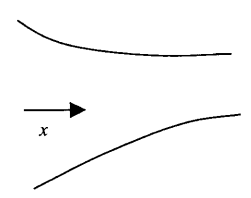
\includegraphics[width=.65\columnwidth]{figs/B/fig3.png}
  \caption{Diagram}
  \label{fig:figs/B/fig3.png}
\end{figure}

\hfill{(GATE 2011 XE)} \\
\begin{multicols}{4}
(A) $50(x + x^3)$\\
(B) $50(1 + x^2)$\\
(C) $0$\\
(D) $50(x^2 + x^3)$
\end{multicols}

\item Consider fully developed flow of water in a pipe of diameter 2 cm. The average velocity of the flow is 2 m/s. The viscosity of the water is $10^{-3}$ kg/m-s and the density is 1000 kg/m$^3$. The friction factor can be calculated using $f = 64/\mathrm{Re}$ for laminar flows and $f = 0.3164/\mathrm{Re}^{0.25}$ for turbulent flows. The pressure drop over a length of 0.5 m is\\

\hfill{(GATE 2011 XE)} \\
\begin{multicols}{4}
(A) 0.08 Pa\\
(B) 325 Pa\\
(C) 1115 Pa\\
(D) 9875 Pa
\end{multicols}

\item Consider a steady, fully developed flow in a horizontal pipe of diameter D. Over a section of length L of this pipe, a pressure drop of $\Delta p$ is observed. The average wall shear stress over this section is\\

\hfill{(GATE 2011 XE)} \\
\begin{multicols}{4}
(A) $\frac{\Delta p D}{4L}$\\
(B) $\frac{\Delta p D}{2L}$\\
(C) $\frac{\Delta p \pi}{2D}$\\
(D) $\frac{\Delta p \pi}{4D}$
\end{multicols}

\newpage

\item In an inviscid incompressible flow, the velocity field is given by $\mathbf{V} = x \mathbf{i} + y \mathbf{j}$ m/s and the body force per unit mass is given by $g = -10 \mathbf{k}$ m/s$^2$. The pressure at the point (0, 0, 0) is 101 Pa. Assuming that the density of the fluid is 1 kg/m$^3$, the pressure at the point (1, 1, 1) for this flow is\\

\hfill{(GATE 2011 XE)} \\
\begin{multicols}{4}
(A) 100 Pa\\
(B) 105 Pa\\
(C) 95 Pa\\
(D) 90 Pa
\end{multicols}


\item[\textbf{Q17 \& Q18:}]
A two-dimensional rectangular water jet of velocity 10 m/s and area 5 cm$^2$ impinges normal to a flat plate and splits symmetrically into two half jets, each of area 2.5 cm$^2$ as shown. Assume steady flow and neglect viscous effects and the weight of the plate and the water. Density of water is 1000 kg/m$^3$.\\

\begin{figure}[htbp]
  \centering
  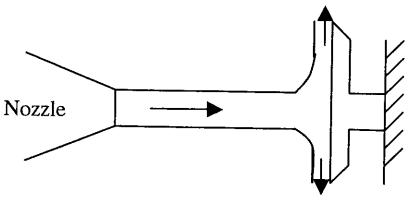
\includegraphics[width=.65\columnwidth]{figs/B/fig4.png}
  \caption{Water Jet Diagram}
  \label{fig:figs/B/fig4.png}
\end{figure}

\item[17.] After splitting, the velocity of the upward half-jet along the plate is\\

\hfill{(GATE 2011 XE)} \\
\begin{multicols}{4}
(A) 5 m/s\\
(B) 7.5 m/s\\
(C) 2.5 m/s\\
(D) 10 m/s
\end{multicols}

\item[18.] The magnitude of the reaction force at the wall is\\

\hfill{(GATE 2011 XE)} \\
\begin{multicols}{4}
(A) 20 N\\
(B) 25 N\\
(C) 35 N\\
(D) 50 N
\end{multicols}

\newpage 
 
\item[\textbf{Q19 \& Q20:}]
A flow has a velocity field given by $\mathbf{V} = 2x \mathbf{i} - 2y \mathbf{j}$.\\

\item[19.] The velocity potential $\phi(x, y)$ for the flow is\\

\hfill{(GATE 2011 XE)} \\
\begin{multicols}{4}
(A) $2x - 2y + \text{const.}$\\
(B) $2xy + \text{const.}$\\
(C) $x^2 + y^2 + \text{const.}$\\
(D) $x^2 - y^2 + \text{const.}$
\end{multicols}

\item[20.] The streamlines for the velocity field look like\\

\hfill{(GATE 2011 XE)} \\
\begin{multicols}{4}
(A) 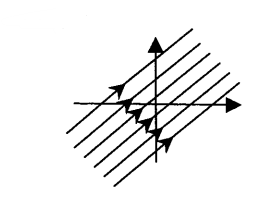
\includegraphics[height=2.5cm]{figs/B/fig20a.png} \\
(B) 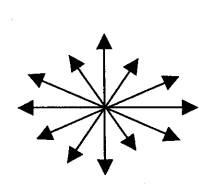
\includegraphics[height=2.5cm]{figs/B/fig20b.png} \\
(C) 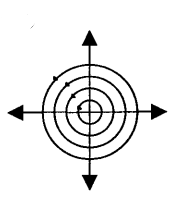
\includegraphics[height=2.5cm]{figs/B/fig20c.png} \\
(D) 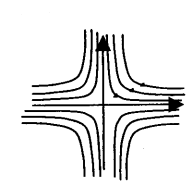
\includegraphics[height=2.5cm]{figs/B/fig20d.png} \\
\end{multicols}

\item[\textbf{Q21 \& Q22:}]

Two flat parallel plates are separated by a small gap $h$ filled with an incompressible fluid of viscosity $\mu$. Assume that the length and width of the plates to be much larger than the gap $h$. The top plate moves horizontally while the bottom plate is held stationary. The magnitude of the difference between the shear stress at the top and bottom walls is found to be $\Delta \tau$.\\


\item[21.] The velocity of the top plate is:\\

\hfill{(GATE 2011 XE)} \\
\begin{multicols}{4}
(A) $\frac{h\Delta\tau}{2\mu}$\\
(B) $\frac{h\Delta\tau}{\mu}$\\
(C) $\frac{2h\Delta\tau}{\mu}$\\
(D) $\frac{3h\Delta\tau}{2\mu}$
\end{multicols}

\item[22.] If a finite width slender object is introduced parallel to the plates in the middle of the gap, the time at which it would have rotated clockwise by $90^\circ$ would be:\\

\hfill{(GATE 2011 XE)} \\
\begin{multicols}{4}
(A) $\frac{2\pi\mu}{\Delta\tau}$\\
(B) $\frac{\pi\mu}{\Delta\tau}$\\
(C) $\frac{2\pi\mu}{3\Delta\tau}$\\
(D) $\frac{\pi\mu}{4\Delta\tau}$
\end{multicols}

\end{enumerate}

\vspace{1\baselineskip}
    \begin{center}
    \textbf{\Large END OF SECTION- B}
    \end{center}


%---------------------SECTION-C--------------------------------
\newpage
\section{C: Material Science}

\begin{enumerate}

\item Which one of the following pairs of crystal structures can have the same packing fraction of 0.74?

\hfill{(GATE 2011 XE)}\\
\begin{multicols}{4}
(A) FCC and BCC \\
(B) HCP and BCC \\
(C) FCC and HCP \\
(D) BCC and BCT
\end{multicols}

\item Which one of the following is NOT CORRECT?

\hfill{(GATE 2011 XE)}\\
\begin{multicols}{2}
(A) An edge dislocation can cross slip \\
(B) An edge dislocation can glide \\
(C) A screw dislocation can cross slip \\
(D) An edge dislocation can climb
\end{multicols}

\item Which one of the following is NOT CORRECT?

\hfill{(GATE 2011 XE)}\\
\begin{multicols}{2}
(A) Working of lead at 25$^\circ$C is hot working \\
(B) Working of tungsten at 1000$^\circ$C is hot working \\
(C) Working of lead at $-100^\circ$C is cold working \\
(D) Working of tungsten at 25$^\circ$C is cold working
\end{multicols}

\item Which one of the following is NOT a ceramic?

\hfill{(GATE 2011 XE)}\\
\begin{multicols}{4}
(A) SiC \\
(B) MgO \\
(C) TiB$_2$ \\
(D) TiAl
\end{multicols}

\item If the average degree of polymerisation of a polyvinyl chloride (PVC) polymer is 2000, then its average molecular weight (in g mol$^{-1}$) is

\hfill{(GATE 2011 XE)}\\
\begin{multicols}{4}
(A) 125000 \\
(B) 119000 \\
(C) 56000 \\
(D) 2000
\end{multicols}

\item Which one of the following materials has the lowest coefficient of thermal expansion?

\hfill{(GATE 2011 XE)}\\
\begin{multicols}{4}
(A) Superalloy \\
(B) Super Invar \\
(C) Spinel \\
(D) $\alpha$-brass
\end{multicols}


\item The colour of a metal is determined by the wavelength distribution of the radiation that is

\hfill{(GATE 2011 XE)}\\
\begin{multicols}{4}
(A) diffracted \\
(B) transmitted \\
(C) reflected \\
(D) refracted
\end{multicols}

\newpage

\item Nickel ferrite is

\hfill{(GATE 2011 XE)}\\
\begin{multicols}{4}
(A) antiferromagnetic \\
(B) ferromagnetic \\
(C) diamagnetic \\
(D) ferrimagnetic
\end{multicols}

\item The oxide scale responsible for the excellent corrosion resistance of stainless steels is

\hfill{(GATE 2011 XE)}\\
\begin{multicols}{4}
(A) Cr$_2$O$_3$ \\
(B) NiO \\
(C) Fe$_2$O$_3$ \\
(D) FeO
\end{multicols}

\item Match the properties in Column-I with the appropriate units in Column-II.

\begin{center}
\begin{tabular}[12pt]{|l|l|}
\hline 
  P.Processes   & 1.Characteristics / Applications \\ \hline
  Q.Gas Metal Arc Welding    & 2.Joining of thick plates \\ \hline
  R.Tungsten Inert Gas Welding &  3.Consumable electrode wire  \\ \hline
  S.Electroslag Welding & 4.Joining of cylindrical dissimilar materials \\ \hline
\end{tabular}
\end{center}

\hfill{(GATE 2011 XE)}\\
\begin{multicols}{2}
(A) P–6, Q–4, R–2, S–5 \\
(B) P–3, Q–5, R–1, S–4 \\
(C) P–3, Q–4, R–1, S–5 \\
(D) P–6, Q–5, R–1, S–4
\end{multicols}

\item It takes 4 h for carburising a steel at 900$^\circ$C. If the same carburising is to be accomplished in 2 h, what should be the temperature? The activation energy of diffusion of carbon in steel is 151 kJ~mol$^{-1}$.
(Give the answer to the nearest degree Celsius.)

\hfill{(GATE 2011 XE)}\\


\item A steel specimen (12 mm diameter and 60 mm length) undergoes elastic deformation under tension. The deformed specimen experiences a longitudinal strain of 0.001. If the Poisson's ratio is 0.3, the diameter of the deformed specimen (in mm) is

\hfill{(GATE 2011 XE)}\\
\begin{multicols}{4}
(A) 12.0120 \\
(B) 12.0036 \\
(C) 11.9964 \\
(D) 11.9880
\end{multicols}

\newpage

\item[\textbf{Q13 \& Q14:}] The first peak in the powder X-ray diffraction pattern of an FCC metal appears at a Bragg angle of 19.2$^{\circ}$. The wavelength of Cu-K$\alpha$ radiation used is 0.154 nm.

\item[13)] The lattice parameter of the metal (in nm) is

\hfill{(GATE 2011 XE)}\\
\begin{multicols}{4}
(A) 0.4505 \\
(B) 0.4055 \\
(C) 0.3505 \\
(D) 0.3055
\end{multicols}

\item[14)] The full width at half maximum (FWHM) of the first peak is 0.35$^{\circ}$. Ignoring micro-strain and instrumental broadening, the crystallite size of the sample (in nm) is

\hfill{(GATE 2011 XE)}\\
\begin{multicols}{4}
(A) 20 \\
(B) 24 \\
(C) 200 \\
(D) 240
\end{multicols}

\item[\textbf{Q15 \& Q16:}] For an intrinsic semiconductor, the mobilities of free electrons and holes are 0.14 m$^2$~V$^{-1}$~s$^{-1}$ and 0.038 m$^2$~V$^{-1}$~s$^{-1}$, respectively. Its bandgap is 1.107 eV and electrical conductivity at 300~K is $3.99 \times 10^{-4}$~$\Omega^{-1}$~m$^{-1}$.


\item[15)] The free electron concentration (in m$^{-3}$) at 300~K is

\hfill{(GATE 2011 XE)}\\
\begin{multicols}{4}
(A) $13.99 \times 10^{15}$ \\
(B) $27.98 \times 10^{15}$ \\
(C) $13.99 \times 10^{17}$ \\
(D) $27.98 \times 10^{17}$
\end{multicols}

\item[16)] What is the temperature at which the conductivity of the semiconductor is $0.399~\Omega^{-1}$~m$^{-1}$?

\hfill{(GATE 2011 XE)}\\
\begin{multicols}{4}
(A) 343~K \\
(B) 443~K \\
(C) 493~K \\
(D) 543~K
\end{multicols}

\item[\textbf{Q17 \& Q18:}] A continuous and aligned glass fibre reinforced composite has a modulus of elasticity of 150~GPa in the longitudinal direction. The matrix is a polyester resin with a modulus of 4.5~GPa. The glass fibre has a modulus of 340~GPa.\\


\item[17)] The volume fraction of the glass fibres is

\hfill{(GATE 2011 XE)}\\
\begin{multicols}{4}
(A) 0.398 \\
(B) 0.434 \\
(C) 0.497 \\
(D) 0.566
\end{multicols}

\item[18)] If the cross-sectional area of the composite is 300~mm$^2$, and a stress of 100~MPa is applied in the longitudinal direction, what will be the total load (in kN) carried by the glass fibres?
\hfill{(GATE 2011 XE)}\\
\begin{multicols}{4}
(A) 0.5 \\
(B) 5 \\
(C) 20.5 \\
(D) 29.5
\end{multicols}

\newpage
\item[19)] A hardness test on a particular material gives a Brinell Hardness Number of 200. This means the indentation has happened under a load of 3000 kgf and the diameter of the steel ball used is

\hfill{(GATE 2011 XE)}\\
\begin{multicols}{4}
(A) 2.5 mm \\
(B) 5 mm \\
(C) 10 mm \\
(D) 12.5 mm
\end{multicols}


\item[20)] A composite slab consists of two materials A and B joined in parallel. The thermal conductivities of A and B are $k_A$ and $k_B$, and heat flows perpendicular to the join. If the thicknesses of both slabs are the same and the ratio of their widths is $w_A : w_B = 1:2$, the effective thermal conductivity of the composite is

\hfill{(GATE 2011 XE)}\\
\begin{multicols}{4}
(A) $\frac{k_A + 2k_B}{3}$ \\
(B) $\frac{2k_A + k_B}{3}$ \\
(C) $\frac{k_A k_B}{k_A + 2k_B}$ \\
(D) $\frac{2k_A k_B}{k_B + 2k_A}$
\end{multicols}

\end{enumerate}


\vspace{3\baselineskip}
    \begin{center}
    \textbf{\Large END OF SECTION- C}
    \end{center}

%--------------------SECTION-D---------------------------------
\newpage

\section*{D: Polymer Science and Engineering}
\vspace{1cm}
\begin{enumerate}[label=\arabic*)]

\item Monomers that undergo free radical polymerization have\\

\hfill{(GATE 2011 XE)} \\
\begin{multicols}{2}
(A) one hydroxyl and one carboxylic group\\
(B) double bonds\\
(C) one amine group and one carboxylic group\\
(D) two amine groups
\end{multicols}

\item In the polymerization of phthalic anhydride (3 moles) and glycerol (3 moles), the average functionality of the reacting system is\\

\hfill{(GATE 2011 XE)} \\
\begin{multicols}{4}
(A) 1.2\\
(B) 4.2\\
(C) 3.8\\
(D) 2.5
\end{multicols}

\item A mixture consists of 10 moles of dimer, 15 moles of trimer, 20 moles of tetramer and 5 moles of pentamer. The average chain length of the mixture is\\

\hfill{(GATE 2011 XE)} \\
\begin{multicols}{4}
(A) 3.4\\
(B) 8.5\\
(C) 6.8\\
(D) 1.7
\end{multicols}


\item Polyurethane is formed by\\

\hfill{(GATE 2011 XE)} \\
\begin{multicols}{2}
(A) self condensation of polyols\\
(B) self condensation of diisocyanate\\
(C) reaction of polyol and diisocyanate\\
(D) reaction of polyol with adipic acid
\end{multicols}


\item The glass transition temperature ($T_g$) is governed by\\

\hfill{(GATE 2011 XE)} \\
\begin{multicols}{2}
(A) translational motion of entire molecule\\
(B) long cooperative wriggling motion of 40 to 50 C–C bonds\\
(C) short cooperative motion of 5 to 6 bonds of the molecules\\
(D) vibration of carbon atoms of the polymer molecules
\end{multicols}

\newpage 

\item The miscibility in binary polymer blends of polyvinyl fluoride and polyacrylate is governed by which one of the following interactions?\\

\hfill{(GATE 2011 XE)} \\
\begin{multicols}{4}
(A) dipole-dipole\\
(B) acid-base type\\
(C) hydrogen bonding\\
(D) ion–dipole
\end{multicols}



\item The melting temperature of polytetrafluoroethylene is higher than its degradation temperature due to\\

\hfill{(GATE 2011 XE)} \\
\begin{multicols}{4}
(A) hydrogen bonding\\
(B) $\pi$-hydrogen bonding\\
(C) van der Waal’s interaction\\
(D) dipole moment interaction
\end{multicols}

\item As the molecular weight (M) increases beyond the critical molecular weight ($M_c$), the zero shear viscosity of a polymer melt becomes proportional to\\

\hfill{(GATE 2011 XE)} \\
\begin{multicols}{4}
(A) $M^{0.5}$\\
(B) $M^{3.4}$\\
(C) $M^{1.0}$\\
(D) $M^0$
\end{multicols}

\item In the step-growth polymerization of phenol with formaldehyde, the functionality of phenol is\\

\hfill{(GATE 2011 XE)} \\
\begin{multicols}{4}
(A) 2\\
(B) 5\\
(C) 4\\
(D) 3
\end{multicols}



\item During the processing of polymers, degradation occurs. Pair each item in Column-I with the appropriate one in Column-II.

\begin{table}[htbp]
  \centering
  \caption{Table-3}
  \label{table3}
  \begin{tabular}{cc}

\textbf{Column I} & \textbf{Column II}\\
     (P) Solid state sintering & (1) Carbon nanotube products\\
     (Q) Liquid phase sintering & (2) Mixture of Cu and Zn powder\\
     (R) Spark plasma sintering & (3) iron powder products\\
     (S) Laser sintering & (4) 3D printed products

  \end{tabular}
\end{table}


\hfill{(GATE 2011 XE)} \\
\begin{multicols}{2}

(A) P-1, Q-3, R-2, S-4\\
(B) P-1, Q-2, R-3, S-4\\
(C) P-2, Q-1, R-3, S-4\\
(D) P-4, Q-2, R-3, S-1
\end{multicols}

\newpage

\item The solubility parameter of polystyrene is $9.1\,(\text{cal/cm}^3)^{1/2}$, the solubility parameter of n-hexane is $7.3\,(\text{cal/cm}^3)^{1/2}$ and that of benzene is $9.2\,(\text{cal/cm}^3)^{1/2}$. Then polystyrene will\\

\hfill{(GATE 2011 XE)} \\
\begin{multicols}{2}
(A) dissolve in n-hexane\\
(B) not dissolve in 80:20 mixture of n-hexane and benzene\\
(C) not dissolve in benzene\\
(D) dissolve in benzene
\end{multicols}

\item Fibre glass composites are prepared by coating unidirectional fibre glass with epoxy prepolymer. If slippage DOES NOT occur at the interface in the loading in the direction of fibre, then\\

\hfill{(GATE 2011 XE)} \\
\begin{multicols}{2}
(A) force sheared by fibre glass ($P_f$) and matrix ($P_m$) should be equal\\
(B) strain as well as force in fibre ($\epsilon_f$, $P_f$) are both equal to strain and the force in matrix ($\epsilon_m$, $P_m$)\\
(C) strain at the interface between fibre glass ($\epsilon_f$) and matrix ($\epsilon_m$) should be equal\\
(D) None of the above is true
\end{multicols}

\item The power factor (PF) and dissipative factor (DF) of polymeric materials are related by\\

\hfill{(GATE 2011 XE)} \\
\begin{multicols}{4}
(A) PF = DF/$(1 - DF^2)^{1/2}$\\
(B) DF = PF/$(1 - PF^2)^{1/2}$\\
(C) DF = $1/(1 - PF^2)^{1/2}$\\
(D) PF = $1/(1 - DF^2)^{1/2}$
\end{multicols}

\item Poly methyl methacrylate (PMMA) and silicone can be used respectively in\\

\hfill{(GATE 2011 XE)} \\
\begin{multicols}{2}
(A) medical syringe and hip joint\\
(B) soft tissue replacement and contact lenses\\
(C) hip joint and medical syringe\\
(D) contact lenses and soft tissue replacement
\end{multicols}

\item In the log (viscosity) versus log (shear rate) behaviour of polymer melts, the upper ($\mu_{upper}$) and lower ($\mu_{lower}$) Newtonian viscosities are related as\\

\hfill{(GATE 2011 XE)} \\
\begin{multicols}{2}
(A) $\mu_{upper}$ and $\mu_{lower}$ versus shear rate are connected by discontinuous curve\\
(B) $\mu_{upper} > \mu_{lower}$\\
(C) $\mu_{upper} < \mu_{lower}$\\
(D) $\mu_{upper} = \mu_{lower}$
\end{multicols}

\newpage

\item Match the following additives for plastic with their respective functions.

\begin{center}
\begin{tabular}{lcc}
 & {Automat} & {Center Lathe} \\
\hline
Machine Setup Time (min) & 120 & 30 \\ \hline
Machine Setup Cost (Rs./min) & 800 & 150 \\ \hline
Machining Time per piece (min) & 2 & 25 \\ \hline
Machining Cost (Rs./min) & 500 & 100 \\ \hline \\
\end{tabular}
\end{center}

\hfill{(GATE 2011 XE)} \\
\begin{multicols}{2}

(A) P-1, Q-2, R-3, S-4\\
(B) P-3, Q-4, R-2, S-1\\
(C) P-3, Q-2, R-1, S-4\\
(D) P-4, Q-3, R-2, S-1
\end{multicols}

% Common Data for Q17 & Q18

\item[\textbf{Q17 \& Q18:}] In a single-screw extruder the dimensions of the channel are: Diameter (D) = 5.03 cm, Width (W) = 1.1 cm, Height (H) = 0.36 cm, Screw Angle ($\theta$) = 6.3$^\circ$ and Speed of Rotation = 10 revolutions per second (rps).\\

\item Assume a flat plate model in the melt zone of a single-screw extruder
$
\frac{\partial P}{\partial z} = \frac{\partial^2 v_z}{\partial y^2};\quad v_z = 0 \text{ at } y=0, \ v_z = V_{bz} \text{ at } y=H$
For fully developed flow in the z direction $v_z$ is found to be\\

\hfill{(GATE 2011 XE)} \\
\begin{multicols}{2}
(A) $v_z = V_{bz}(y/H) - [y(H-y) \frac{\partial P}{\partial z}]/(2\eta)$\\
(B) $v_z = (y/H) + [y(H-y) \frac{\partial P}{\partial z}]/(2\eta)$\\
(C) $v_z = (y^2/H) + [y(H-y) \frac{\partial P}{\partial z}]/(2\eta)$\\
(D) $v_z = (y^2/H) - [y(H-y) \frac{\partial P}{\partial z}]/(2\eta)$
\end{multicols}

\item In the absence of a die in a single screw extruder $\Delta P = 0$ and $Q$ is equal to\\

\hfill{(GATE 2011 XE)} \\
\begin{multicols}{4}
(A) 0.31 cm$^3$/sec\\
(B) 3.11 cm$^3$/sec\\
(C) 311 cm$^3$/sec\\
(D) 31.1 cm$^3$/sec
\end{multicols}

% Common Data for Q19 & Q20
\item[\textbf{Q19 \& Q20:}] In the polymerization of styrene at 60$^\circ$C, it is assumed that all steps are irreversible and\\
-- propagation rate constant ($k_p$) = 145 lit/mol-sec\\
-- mutual termination rate constant ($k_t$) = 0.13 $\times$ 10$^7$ lit/mol-sec\\
-- initiator rate constant ($k_I$) = 4.38 $\times$ 10$^6$ sec$^{-1}$\\
-- initiator concentration ([I$_2$]) = 1.65 $\times$ 10$^2$ mol/liter\\
-- monomer concentration ([M]) = 7.69 mol/liter\\

\item Assuming the rate constant for combination of initiator radical with monomer, $k_1 = 10 k_t$, in the polymerization of styrene, the primary radical concentration ([I]) can be calculated as\\

\hfill{(GATE 2011 XE)} \\
\begin{multicols}{4}
(A) $[I] = 0.364 \times 10^0$ mol/lit\\
(B) $[I] = 1.65 \times 10^{-10}$ mol/lit\\
(C) $[I] = 6.48 \times 10^{-12}$ mol/lit\\
(D) $[I] = 2.74 \times 10^4$ mol/lit
\end{multicols}

\item The total molar concentration of the growing polymer radicals ($\rho$) in the polymerization of styrene is given by\\

\hfill{(GATE 2011 XE)} \\
\begin{multicols}{4}
(A) $\rho = 4.72 \times 10^8$ mol/lit\\
(B) $\rho = 2.36 \times 10^7$ mol/lit\\
(C) $\rho = 7.08 \times 10^6$ mol/lit\\
(D) $\rho = 9.44 \times 10^5$ mol/lit
\end{multicols}

% Linked Answer Questions (21 & 22)

\item[\textbf{Q21 \& Q22:}] For semi-crystalline polymeric materials, free of voids and impurities, we define the following:\\
$\rho$ = average density of a semi-crystalline polymer\\
$\rho_c$ = density of the crystalline phase\\
$\rho_a$ = density of the amorphous phase\\

\item The relation between the average density and the densities of crystalline and amorphous phases can be related to mass fraction of the crystalline phase (X) as:\\

\hfill{(GATE 2011 XE)} \\
\begin{multicols}{4}
(A) $(1/\rho) = (X/\rho_c) + (1/\rho_a)$\\
(B) $(1/\rho) = (1/\rho_c) + (1/\rho_a)$\\
(C) $(1/\rho) = (1/\rho_c) + \{(1 - X)/\rho_a\}$\\
(D) $(1/\rho) = (X/\rho_c) + \{(1 - X)/\rho_a\}$
\end{multicols}

\item When a fiber is made of PET, it has crystalline as well as amorphous phases and experiments have revealed that the average density of the overall material is 1.375 g/cm$^3$. It is known that the density of the crystalline phase is 1.455 g/cm$^3$ and that of amorphous phase is 1.335 g/cm$^3$. The mass fraction crystallinity (X) in \% is given by:\\

\hfill{(GATE 2011 XE)} \\
\begin{multicols}{4}
(A) 35.3\%\\
(B) 50.5\%\\
(C) 80.1\%\\
(D) 5.1\%
\end{multicols}
\end{enumerate}

\vspace{3\baselineskip}
    \begin{center}
    \textbf{\Large END OF SECTION- D}
    \end{center}

%----------------------SECTION-E-------------------------------------
\newpage

\section*{E: Food Technology}
\vspace{1cm}

\begin{enumerate}

\item The protein responsible for spongy structure in bread is

\hfill{(GATE 2011 XE)} \\
\begin{multicols}{4}
(A) Albumin \\
(B) Zein \\
(C) Gluten \\
(D) Gliadin
\end{multicols}


\item The factor most responsible for making a good ice cream is

\hfill{(GATE 2011 XE)} \\
\begin{multicols}{4}
(A) Water content \\
(B) Homogenization \\
(C) Emulsifying agent \\
(D) Mixing index
\end{multicols}

\item Listed below are some of the functions of fats in the human nutrition. Identify the INCORRECT function.

\hfill{(GATE 2011 XE)} \\
\begin{multicols}{2}
(A) Concentrated source of energy \\
(B) Transport of oxygen to various organs \\
(C) Absorption of fat soluble vitamins \\
(D) Synthesis of cell membranes and hormones
\end{multicols}

\item During ripening of cheese by Penicillium roqueforti the characteristic aroma is because of

\hfill{(GATE 2011 XE)} \\
\begin{multicols}{4}
(A) Methyl ketones \\
(B) Aceto acetic acid \\
(C) Diacetyl \\
(D) Acetoin
\end{multicols}

\item Which of the following statements is NOT TRUE in case of oxidative rancidity of fatty foods?

\hfill{(GATE 2011 XE)} \\

(A) Peroxides and hydroperoxides are formed during auto-oxidation \\
(B) Auto-oxidation is a complex chain reaction \\
(C) The final breakdown products of auto-oxidation are aldehydes, ketones and alcohols \\
(D) The reaction is brought about by an enzyme, called lipase


\item Which of the following group of characteristics is CORRECT in respect of Shigella species found as food pathogen?

\hfill{(GATE 2011 XE)} \\

(A) Gram positive, motile by gliding, spore forming cocci and transmitted by contaminated food \\
(B) Gram negative, motile by flagella, spore forming bacilli and transmitted by contaminated water \\
(C) Gram positive, non-motile, non-spore forming cocci and transmitted by contaminated air and water both \\
(D) Gram negative, non-motile, non-spore forming and transmitted by fecal-oral route

\newpage

\item Relate the vitamins listed below (left hand side) with the associated diseases (right hand side):\\

\begin{table}
\begin{center}
\begin{tabular}{|c|c|c|c|c|}
\hline
\textbf{Q.No.} & \textbf{Type} & \textbf{Section} & \textbf{Key} & \textbf{Marks} \\
\hline
1  & MCQ & PI & C                & 1 \\ \hline
2  & MCQ & PI & D                & 1 \\ \hline
3  & MCQ & PI & A                & 1 \\ \hline
4  & MCQ & PI & D                & 1 \\ \hline
5  & MCQ & PI & B                & 1 \\ \hline
6  & MCQ & PI & A                & 1 \\ \hline
7  & NAT & PI & 1.4 to 1.4       & 1 \\ \hline
8  & MCQ & PI & B                & 1 \\ \hline
9  & NAT & PI & 0.41 to 0.42     & 1 \\ \hline
10 & MCQ & PI & B                & 1 \\ \hline
11 & MCQ & PI & C                & 1 \\ \hline
12 & MCQ & PI & C                & 1 \\ \hline
13 & MCQ & PI & C                & 1 \\ \hline
14 & MCQ & PI & A                & 1 \\ \hline
15 & NAT & PI & 384 to 385       & 1 \\ \hline
16 & MCQ & PI & C                & 1 \\ \hline
17 & MCQ & PI & C                & 1 \\ \hline
18 & MCQ & PI & C                & 1 \\ \hline
19 & NAT & PI & 1.80 to 1.85     & 1 \\ \hline
20 & MCQ & PI & D                & 1 \\ \hline
21 & MCQ & PI & A                & 1 \\ \hline
22 & MCQ & PI & B                & 1 \\ \hline
23 & MCQ & PI & D                & 1 \\ \hline
24 & MCQ & PI & D                & 1 \\ \hline
25 & MCQ & PI & B                & 1 \\ \hline
26 & MCQ & PI & C                & 2 \\ \hline
27 & MCQ & PI & A                & 2 \\ \hline
28 & NAT & PI & 2.2 to 2.3       & 2 \\ \hline
29 & NAT & PI & 70 to 70         & 2 \\ \hline
30 & NAT & PI & 18.00 to 19.00   & 2 \\ \hline
31 & MCQ & PI & A                & 2 \\ \hline
32 & MCQ & PI & C                & 2 \\ \hline
33 & NAT & PI & 2.0 to 2.0       & 2 \\ \hline
34 & NAT & PI & 5.5 to 6.0       & 2 \\ \hline
35 & NAT & PI & 3 to 3           & 2 \\ \hline
36 & MCQ & PI & C                & 2 \\ \hline
37 & MCQ & PI & C & 2 \\ \hline
38 & NAT & PI & 326 to 326 & 2 \\ \hline
39 & NAT & PI & 48 to 48 & 2 \\ \hline
40 & NAT & PI & 2900 to 2900 & 2 \\ \hline
41 & MCQ & PI & A & 2 \\ \hline
42 & NAT & PI & 2.40 to 2.50 & 2 \\ \hline
43 & NAT & PI & 11.00 to 11.20 & 2 \\ \hline
44 & MCQ & PI & D & 2 \\ \hline
45 & NAT & PI & 0.970 to 0.980 & 2 \\ \hline
46 & NAT & PI & 1 to 1 & 2 \\ \hline
47 & MCQ & PI & B & 2 \\ \hline
48 & NAT & PI & 2250.0 to 2265.0 & 2 \\ \hline
49 & MCQ & PI & B & 2 \\ \hline
50 & NAT & PI & 1250 to 1250 & 2 \\ \hline
51 & MCQ & PI & D & 2 \\ \hline
52 & MCQ & PI & A & 2 \\ \hline
53 & NAT & PI & -84 to -80 or 80 to 84 & 2 \\ \hline
54 & NAT & PI & 1.00 to 1.10 & 2 \\ \hline
55 & MCQ & PI & D & 2 \\ \hline
56 & MCQ & GA & A & 1 \\ \hline
57 & MCQ & GA & A & 1 \\ \hline
58 & MCQ & GA & D & 1 \\ \hline
59 & MCQ & GA & B & 1 \\ \hline
60 & MCQ & GA & B & 1 \\ \hline
61 & MCQ & GA & D & 2 \\ \hline
62 & MCQ & GA & A & 2 \\ \hline
63 & MCQ & GA & A & 2 \\ \hline
64 & MCQ & GA & A & 2 \\ \hline
65 & MCQ & GA & C & 2 \\ \hline
\end{tabular}
\end{center}

\end{table}



\hfill{(GATE 2011 XE)} \\
\begin{multicols}{4}
(A) P-1, Q-2, R-3, S-4 \\
(B) P-4, Q-3, R-2, S-1 \\
(C) P-2, Q-1, R-4, S-3 \\
(D) P-3, Q-4, R-1, S-2
\end{multicols}

\item Which of the following conditions for the heat resistance of microorganisms is CORRECT?

\hfill{(GATE 2011 XE)} \\
\begin{multicols}{2}
(A) Psychrophiles $<$ Mesophiles $<$ Thermophiles \\
(B) Psychrophiles $>$ Mesophiles $>$ Thermophiles \\
(C) Thermophiles $>$ Psychrophiles $>$ Mesophiles \\
(D) Mesophiles $<$ Thermophiles $<$ Psychrophiles
\end{multicols}

\item The solubility of sodium bicarbonate in water is 9.6 g/100 g at 20 °C and 16.4 g/100 g at 60 °C. If a saturated solution of sodium bicarbonate at 60 °C is cooled to 20 °C, the percentage of the dissolved salt crystallized out will be

\hfill{(GATE 2011 XE)} \\
\begin{multicols}{4}
(A) 20.5 \% \\
(B) 25.4 \% \\
(C) 41.5 \% \\
(D) 45.2 \%
\end{multicols}

\item A sugar syrup (density = 1040 kg/m³ and viscosity = $1600 \times 10^{-3}$ Pa·s) is required to be pumped into a tank (1.5 m diameter and 3 m height) by a 3 cm inside diameter pipe. If the liquid is required to flow under laminar flow conditions, the minimum time to fill the tank with the syrup will be

\hfill{(GATE 2011 XE)} \\
\begin{multicols}{4}
(A) 192.9 hours \\
(B) 19.3 hours \\
(C) 38.6 hours \\
(D) 57.9 hours
\end{multicols}


\item Match the following sauerkraut defects for their causative agents: \\

\begin{table}[htbp]
  \centering
  \caption{Table-6}
  \label{table6}
  \begin{tabular}{cc}
\textbf{Products} & \textbf{Polymer}\\

P. Electrical cables & 1. Polyurethane \\
Q. Electrical switches & 2. Poly(methyl methacrylate) \\
R. Optical lenses & 3. Cross-linked polyethylene \\
S. Shoe soles & 4. Phenol formaldehyde resin \\
  
  
  
  \end{tabular}
\end{table}

\hfill{(GATE 2011 XE)} \\
\begin{multicols}{2}
(A) P-4, Q-2, R-3, S-1 \\
(B) P-3, Q-4, R-1, S-2 \\
(C) P-1, Q-3, R-2, S-4 \\
(D) P-2, Q-1, R-4, S-3
\end{multicols}

\item Match the following carbohydrates with their use in food processing \\

\begin{center}
\begin{tabular}{|c|c|c|c|c|c|c|c|c|c|c|c|}
\hline
$x$ & 0 & 1 & 2 & 3 & 4 & 5 & 6 & 7 & 8 & 9 & 10 \\
\hline
$y\brak{x}$ & 5 & 3 & 0 & -5 & -10 & -6 & 0 & 5 & 11 & 18 & 30 \\
\hline
\end{tabular}
\end{center}



\hfill{(GATE 2011 XE)} \\
\begin{multicols}{2}
(A) P-1, Q-2, R-4, S-3 \\
(B) P-2, Q-4, R-1, S-3 \\
(C) P-3, Q-1, R-2, S-4 \\
(D) P-4, Q-3, R-1, S-2
\end{multicols}

\item Match the food items and their principal flavouring agents:\\

\begin{center}
    \begin{tabular}{c c c}
    \hline
      {Operation}   & {Precedence} & {Processing time(in min)} \\ \hline
        P & none & 1 \\ \hline
        Q & P & 1\\ \hline
        R & P & 4 \\ \hline
        S & Q,R & 3 \\ \hline 
    \end{tabular}
\end{center}



\hfill{(GATE 2011 XE)} \\
\begin{multicols}{2}
(A) P-3, Q-2, R-4, S-1 \\
(B) P-2, Q-3, R-1, S-4 \\
(C) P-4, Q-1, R-3, S-2 \\
(D) P-4, Q-2, R-3, S-1
\end{multicols}

\item Match the food items with their colloidal nature:\\

\begin{tabular}{c c c}
\hline 
Activity (node $i$ \-- node $j$) & Mean duration (in days) & Standard deviation (in days) \\ \hline
1 \-- 2 & 6 & 1 \\ \hline
1 \-- 3 & 9 & 2 \\ \hline
2 \-- 3 & 2 & 0.5 \\ \hline
2 \-- 4 & 8 & 0.5 \\ \hline
3 \-- 4 & 7 & 1 \\ \hline
3 \-- 5 & 8 & 1 \\ \hline
4 \-- 5 & 4 & 1 \\ \hline
\end{tabular}


\hfill{(GATE 2011 XE)} \\
\begin{multicols}{2}
(A) P-2, Q-1, R-3, S-4 \\
(B) P-4, Q-3, R-2, S-1 \\
(C) P-4, Q-2, R-3, S-1 \\
(D) P-3, Q-4, R-1, S-2
\end{multicols}

\newpage

\item In an actively growing (exponential phase) yeast culture, the cell concentration increased from $10^3$ cells/ml to $10^7$ cells/ml in 4 hours. The doubling time of the yeast is

\hfill{(GATE 2011 XE)} \\
\begin{multicols}{2}
(A) 120 minutes \\
(B) 30 minutes \\
(C) 18 minutes \\
(D) 60 minutes
\end{multicols}

\item The steps followed in Gram's staining of microorganisms are: \\
P. Washing with neutral organic solvent \\
Q. Counter staining with a contrast dye \\
R. Staining with basic dye \\
S. Fixing the colour with a suitable mordant \\ \\
Identify the CORRECT sequence. \\
\hfill{(GATE 2011 XE)} \\
\begin{multicols}{2}
(A) Q → S → R → P \\
(B) P → Q → R → S \\
(C) Q → P → S → R \\
(D) R → S → P → Q
\end{multicols}

\item[\textbf{Q17 \& Q18:}] A continuous dryer was used to dry 12 kg/min of a blanched vegetable containing 50\% moisture (wet weight basis) to give a product containing 10\% moisture. As the dryer could handle feed material with moisture content not more than 25\%, a part of dried material was recycled and mixed with the fresh feed.\\

 \item The evaporation rate in the dryer would be
\hfill{(GATE 2011 XE)} \\
\begin{multicols}{2}
(A) 2.08 kg/min \\
(B) 5.33 kg/min \\
(C) 3.33 kg/min \\
(D) 2.93 kg/min
\end{multicols}

\item The recycle ratio to achieve the drying requirement would be
\hfill{(GATE 2011 XE)} \\
\begin{multicols}{2}
(A) 2.00 \\
(B) 1.25 \\
(C) 1.67 \\
(D) 4.16
\end{multicols}

\item[\textbf{Q19 \& Q20:}] An enzyme has a Km of \(4.7 \times 10^{-5}\) M and Vm is 22 micro moles per litre per min. The enzyme reaction is carried out at a substrate concentration of \(2 \times 10^{-4}\) M.\\

\item The initial reaction velocity for this enzyme catalyzed reaction will be
\hfill{(GATE 2011 XE)} \\
\begin{multicols}{2}
(A) 6.5 micro moles per litre per min \\
(B) 17.8 micro moles per litre per min \\
(C) 13.0 micro moles per litre per min \\
(D) 8.9 micro moles per litre per min
\end{multicols}

\newpage 

\item Addition of a competitive inhibitor (Ki = $3 \times 10^{-4}$ M) at a concentration of $5 \times 10^{-4}$ M to the above reaction system will result in the inhibition of enzymatic reaction by
\hfill{(GATE 2011 XE)} \\
\begin{multicols}{2}
(A) 24.0\% \\
(B) 62.5\% \\
(C) 76.0\% \\
(D) 57.5\%
\end{multicols}

\item[\textbf{Q21 \& Q22:}] The F-value at 121.1 °C, equivalent to 99.9999\% destruction of a strain of \textit{Clostridium botulinum}, is 1.8 minutes.  
(Do and F represent the decimal reduction time and lethality of the destruction process at reference temperature, respectively.)\\


\item The Do value of the organism will be
\hfill{(GATE 2011 XE)} \\\
\begin{multicols}{2}
(A) 10.8 minutes \\
(B) 0.3 minutes \\
(C) 6.0 minutes \\
(D) 0.2 minutes
\end{multicols}

\item The Fo value, based on 12D concept using the Do value of the above organism and a most likely spore load in the product of 100, will be

\hfill{(GATE 2011 XE)} \\
\begin{multicols}{2}
(A) 3.0 minutes \\
(B) 1.2 minutes \\
(C) 1.5 minutes \\
(D) 4.2 minutes
\end{multicols}

\end{enumerate}

\vspace{3\baselineskip}
    \begin{center}
    \textbf{\Large END OF SECTION- E}
    \end{center}

\end{document}